\section{Plankton Identifier(PkID)}

\subsection{主窗口}

打开PkID应用程序,显示的界面上共有5个按钮:“Learning”、“Evaluation”、“Prediction”、“Validation”和“Compilation”(图~\ref{fig: Main window})。这5个部分可以相互独立地运行,但是会有运行的先后顺序。比如“Evaluation”和“Prediction”会用到“Learning”生成的文件,“Validation”用到“Prediction”生成的文件,“Compilation”用到“Validation”所生成的文件。因此,当你第一次使用PkID时你应该首先运行“Learning”。

\begin{figure}[!ht]
\centering
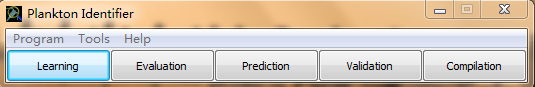
\includegraphics[width=0.8\textwidth]{mainWindow.png}
\caption{主窗口}
\label{fig: Main window}
\end{figure} 

其他菜单:

\textit{\textbf{Program > Settings}} 定义Tanagra.exe所在的路径以及存放缩略图、PID文件和结果的默认文件夹路径。

Tanagra Path:如果你安装了两个以上的Tanagra版本,你可以选择想要使用的版本。点击\textbf{Browse},浏览硬盘文件夹,找到Tanagra.exe,点击\textbf{OK}。

\textit{注:如果你的Tanagra没有安装在 $\backslash$Program Files$\backslash$Tanagra 路径下,或者你就根本没有安装Tanagra,这时当你运行PkID时就会自动弹出这个窗口(图~\ref{fig: Settings window})。}

\begin{figure}[!ht]
\centering
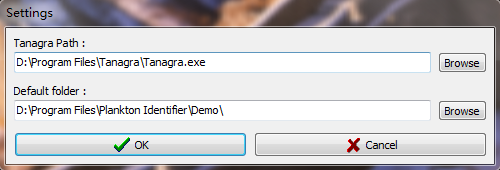
\includegraphics[width=0.7\textwidth]{settingsWindow.png}
\caption{设置窗口}
\label{fig: Settings window}
\end{figure} 

Default folder:默认文件夹是你第一次使用PkID执行一些步骤产生的文件所存放的地方。

\textit{\textbf{Program > Exit}} 关闭PkID。

\subsection{Learning}

这一步会生成一个学习文件以用作后续的自动识别。它对应于经专家鉴定的具有代表性的一些物体的子样本并且可以作为将来分析的参考。

1、文件夹选择窗口

当点击\textbf{Learning}按钮时,会出现如图~\ref{fig: SelectLearningSetFolderWindow}所示的文件夹选择窗口。 

\begin{figure}[!ht]
\centering
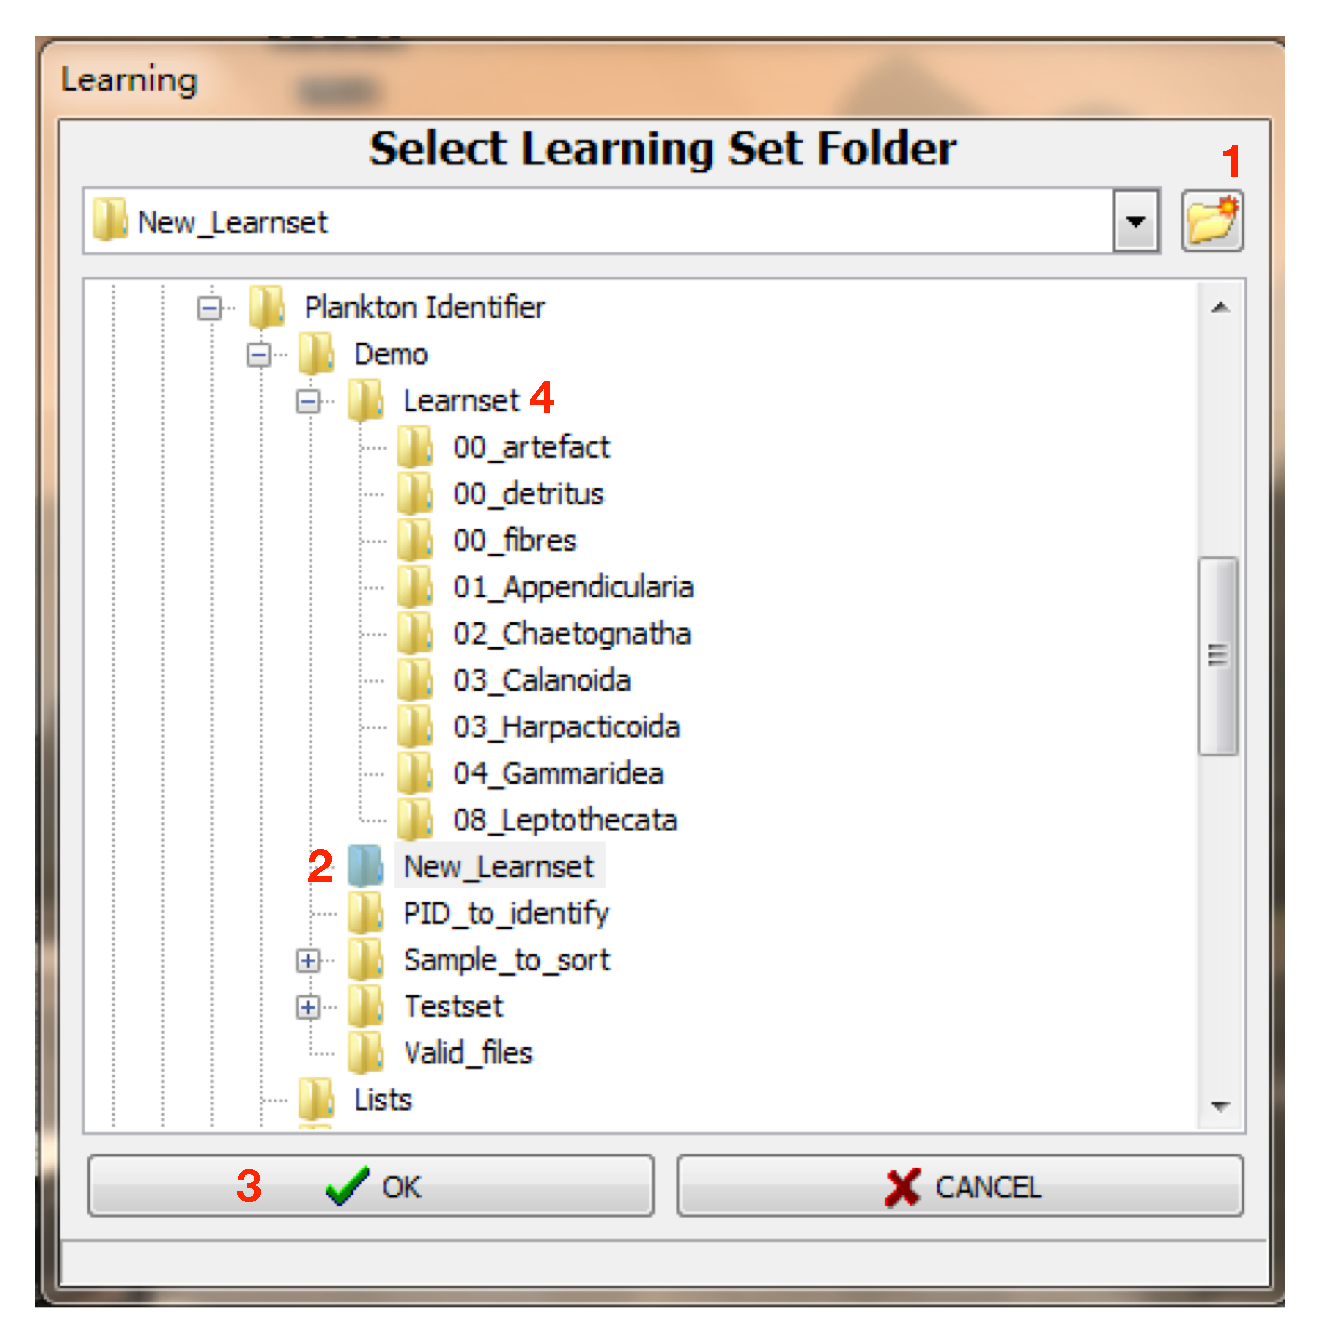
\includegraphics[width=0.6\textwidth]{SelectLearningSetFolderWindow.eps}
\caption{训练集文件夹选择窗口}
\label{fig: SelectLearningSetFolderWindow}
\end{figure} 

选择一个空的文件夹以用来创建新的训练数据集,你也可以通过点击右上角的按钮(图~\ref{fig: SelectLearningSetFolderWindow}: {\color{red}\textbf{1}})来创建一个新的文件夹然后给它命名(图~\ref{fig: SelectLearningSetFolderWindow}: {\color{red}\textbf{2}}),最后点击\textbf{OK}按钮(图~\ref{fig: SelectLearningSetFolderWindow}: {\color{red}\textbf{3}})。

你也可以选择一个已有的训练数据集(其中包含已分类好的子文件夹以及包含物体元数据的一些PID格式的文件,每个子文件夹代表一个种类,其中存放属于该类的jpg格式的缩略图),如图~\ref{fig: SelectLearningSetFolderWindow}: {\color{red}\textbf{4}}。

{\color{blue}\textit{注:如果此处选择的文件夹结构不符,或者包含了无效的数据,那么将会无法打开,并且在窗口的最下方会出现一行红色的警告信息以说明原因。}}

2、学习窗口

当选择了一个可以用来对缩略图进行分类的有效文件夹之后,点击\textbf{OK},会出现一个新的窗口(图~\ref{fig: LearningWindow})。其中左边部分(“Sample Set”)是要通过浏览硬盘文件夹来选择未被分类的样本。右边部分(“Learning Ser”)是要将左边未被分类的样本拖到右边以完成分类(创建子文件夹)。

\begin{figure}[!ht]
\centering
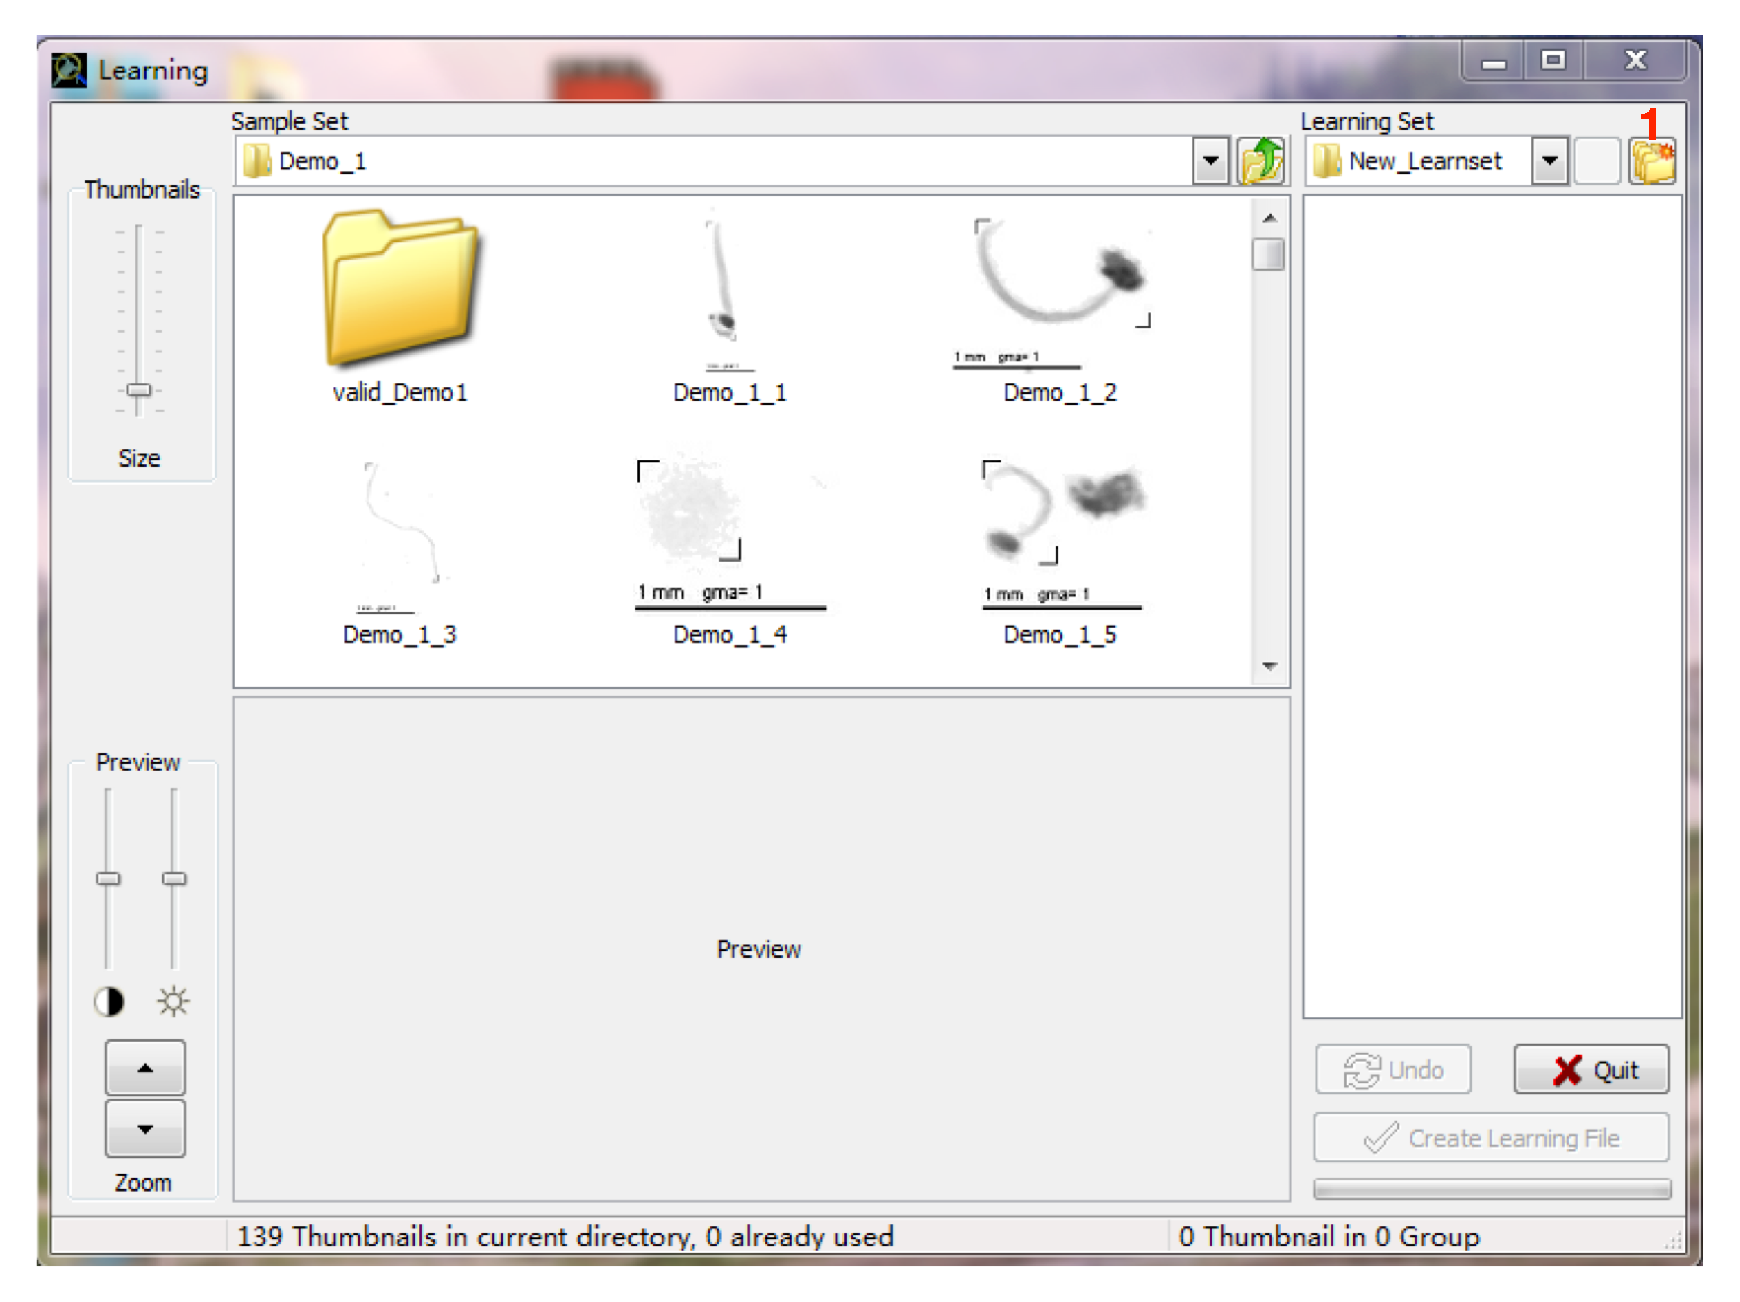
\includegraphics[width=0.6\textwidth]{LearningWindow.eps}
\caption{Learning窗口}
\label{fig: LearningWindow}
\end{figure} 

\textit{Sample Set}

在窗口左边栏“Sample Set”处,浏览硬盘文件夹以打开一个包含未分类的缩略图和相应PID文件的文件夹。只有有有效名字(<Sample Name>\_<Item Number>.jpg)的缩略图才会在左边栏中显示出来。如果名字是有效的但是PID文件中并没有包含该幅图像的一些数据,这时就会这个缩略图上方会出现一个问号并且当把鼠标放在问号上时会有相应的原因解释,这幅图也是无法使用的。

\textit{注:如果此处选择的文件夹结构不符,或者包含了无效的数据,那么将会无法打开,并且在窗口的最下方会出现一行红色的警告信息以说明原因。}

\textit{类别(子文件夹)创建}

在窗口右边栏“Learning Set”处,为了把缩略图归到对应的类别,需要在步骤1所选择的文件夹中创建一些子文件夹,每个文件夹代表一类。点击右上角的按钮(图~\ref{fig: LearningWindow}: {\color{red}\textbf{1}})创建新的文件夹,这时会出现一个新的窗口,可以给新创建的文件夹从给定的种类名字中选择一个(图~\ref{fig: CreateGroupsWindow})。如果给定的这些名字中没有合适的,你还可以选择另一个“Predefined Lists”或者先选择“New”作为名字,之后再在“Learning Set”这一栏中重新编辑命名。

\begin{figure}[!ht]
\centering
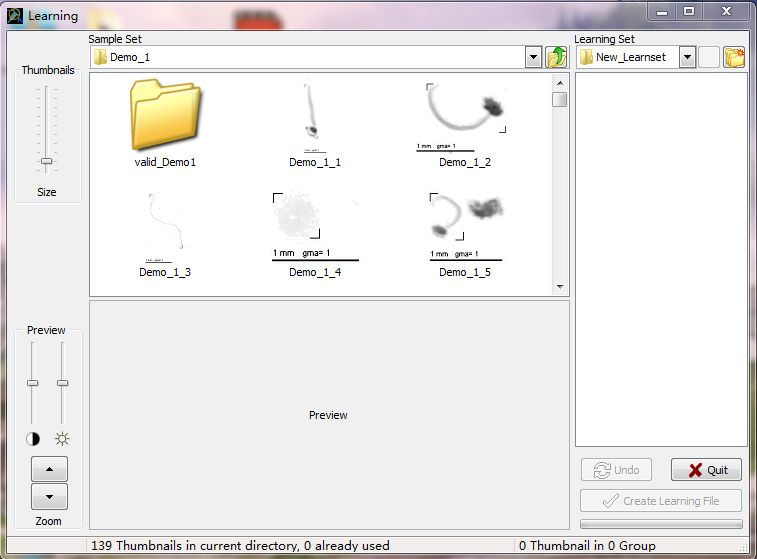
\includegraphics[width=0.6\textwidth]{LearningWindow.png}
\caption{创建训练集中分类类别的窗口}
\label{fig: CreateGroupsWindow}
\end{figure} 

{\color{blue}\textit{注1:所创建的子文件夹名字不能重复。已经用过的名字在“Create Group Folders”窗口中将不再显示。}}

{\color{blue}\textit{注2:可以通过\textbf{Tools>Import Name List}菜单来自定义你自己的种类名字清单。}}

\textit{对缩略图进行归类}

选中一个缩略图,下方会显示它的预览,如图~\ref{fig: ThumbnailsSorting}: {\color{red}\textbf{1}}。你可以通过左侧的\textbf{zoom}按钮(图~\ref{fig: ThumbnailsSorting}: {\color{red}\textbf{2}})将预览结果放大,还可以通过调节左侧对比度和亮度的状态条来显示更多细节。

\begin{figure}[!ht]
\centering
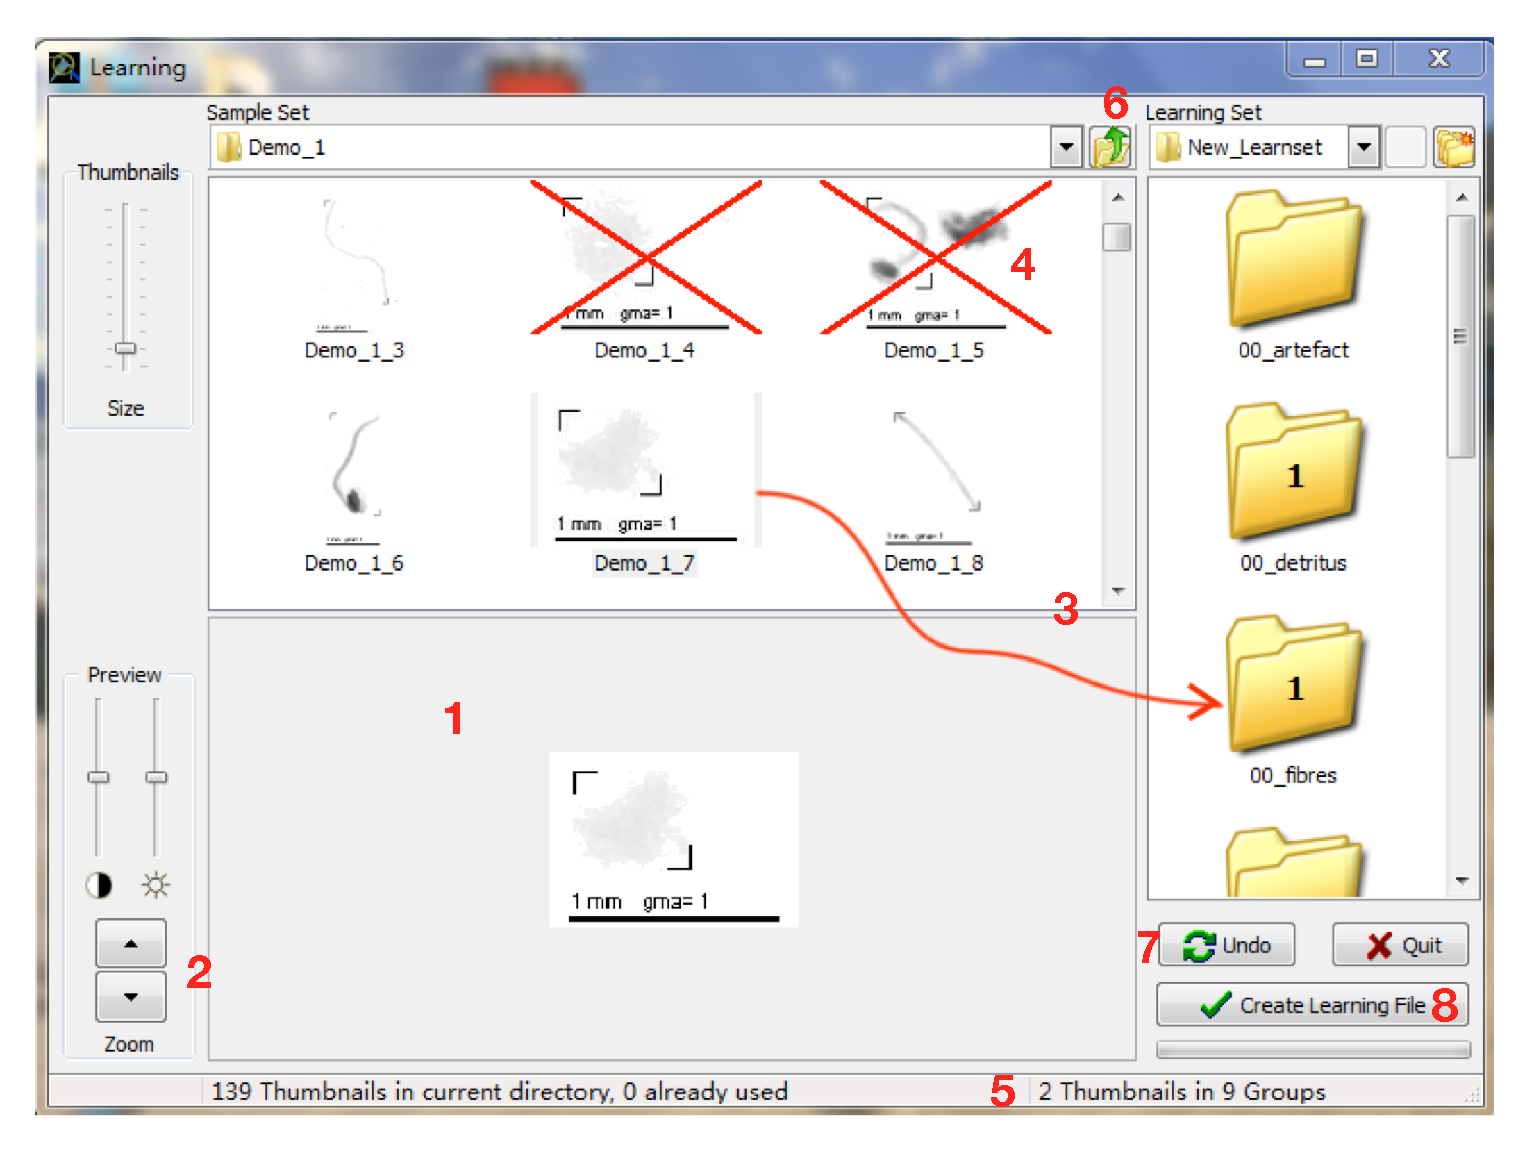
\includegraphics[width=0.7\textwidth]{ThumbnailsSorting.eps}
\caption{对样本文件中的缩略图进行分类}
\label{fig: ThumbnailsSorting}
\end{figure} 

把缩略图拖到相应的子文件夹中(图~\ref{fig: ThumbnailsSorting}: {\color{red}\textbf{3}}),这时缩略图会被复制到那个子文件夹中,而不是被剪切过去了。对应的PID文件也被复制到了右边文件夹中,但在这个窗口中是看不见的,以免视觉上的混淆。一旦一个缩略图已经用在了所创建的数据集中,上面就会出现一个红色的叉(图~\ref{fig: ThumbnailsSorting}: {\color{red}\textbf{4}}),表示它不能再被使用了。

一次选中多个缩略图也是可以的,可以通过按住Ctrl键来完成。在选中多个缩略图的时候,如果你想看每一个缩略图的预览效果,可以从右下角往左上角选择。

每一个子文件夹中缩略图的数目会显示在这个子文件夹上,并且随着你的操作而更新。已经被归类了的缩略图数目以及还没有完成归类的缩略图数目都被显示在了窗口的最下方(图~\ref{fig: ThumbnailsSorting}: {\color{red}\textbf{5}})。

你可以对多个样本集中的缩略图进行归类以创建自己的训练数据集。点击上面的一个按钮(图~\ref{fig: ThumbnailsSorting}: {\color{red}\textbf{6}})转到你想要操作的文件夹路径下。

\textit{Cancel action}

当你在训练数据集的创建过程中执行了一些误操作之后,可以有以下两个办法取消:(1)用\textbf{Undo}按钮(图~\ref{fig: ThumbnailsSorting}: {\color{red}\textbf{7}})(2)打开右侧的子文件夹,选中缩略图然后用DEL键删除。其中\textbf{Undo}键可以用来取消删除操作或子文件夹删除操作,DEL键可以用来删除一个所有缩略图都被清除了的空子文件夹。

\textit{创建学习文件}

一旦你觉得你创建的每一个类别中已经归类了足够多的样本,你就可以点击“Create Learning File”按钮(图~\ref{fig: ThumbnailsSorting}: {\color{red}\textbf{8}})了,点击之后会出现一个保存对话框,上面显示了所要保存的目标文件夹路径以及学习文件的名字,默认的名字为Learn\_<number>格式。点击“Save”按钮,所有的学习工作就完成了。这时又会出来一个会话框询问你是否要继续分类,如果你选择“No”,这个学习窗口就会被关闭回到主窗口。

\subsection{Evaluation}

这一步是要帮助你评估一下基于上一步中创建的训练数据集所建立的预测模型对训练数据集中的物体的识别率有多高。最后会生成一个包含识别结果的文本文件以及一个包含了数据分析信息的html报告。点击主窗口中的Evaluation按钮,会出现如下的界面(图~\ref{fig: EvaluationWindow})。

\begin{figure}[!ht]
\centering
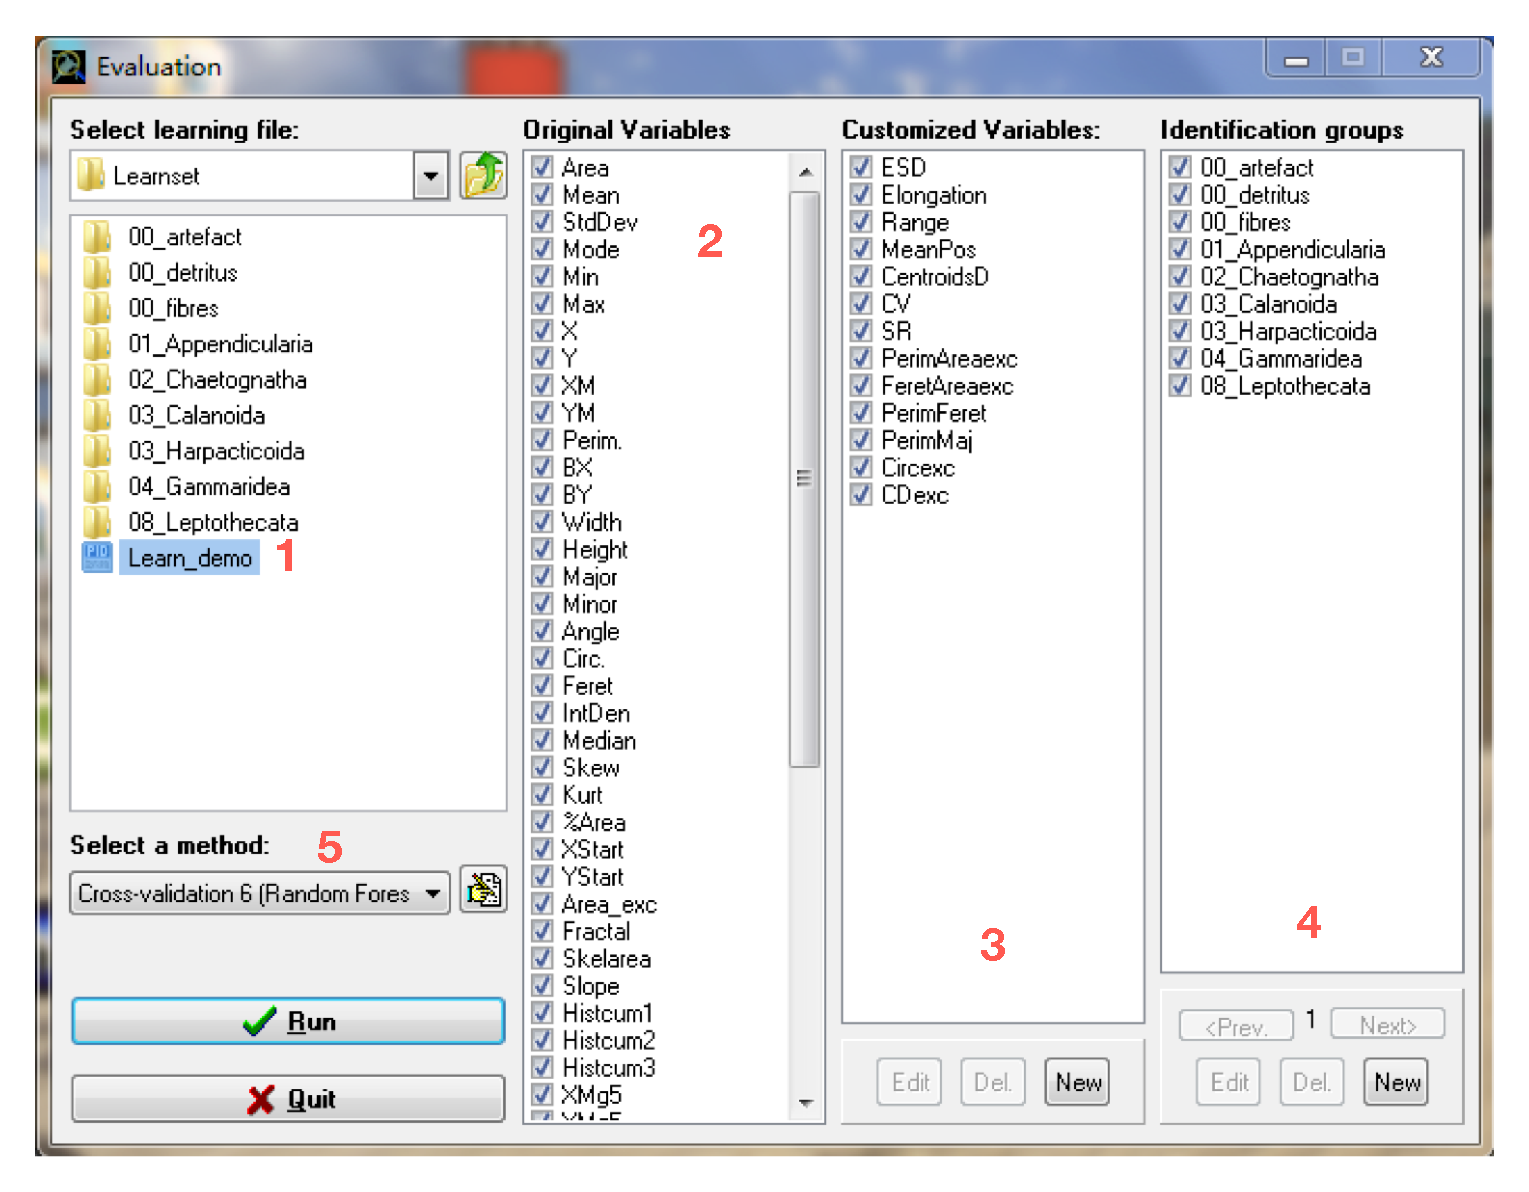
\includegraphics[width=0.7\textwidth]{EvaluationWindow.eps}
\caption{Evaluation窗口}
\label{fig: EvaluationWindow}
\end{figure} 

1、选取学习文件(图~\ref{fig: EvaluationWindow}: {\color{red}\textbf{1}})

浏览硬盘文件夹,选择你想要用来进行数据分析的学习文件。

{\color{blue}\textit{注1:选择学习文件后才能激活其它部分。}}

{\color{blue}\textit{注2:双击PID文件,将会自动在PID viewer(如果已安装)或者文本编辑器(例如Windows下的Notepad)中打开,从而可以校正文件内容。}}

2、初始变量(图~\ref{fig: EvaluationWindow}: {\color{red}\textbf{2}})

这里展示的是所选择的学习文件中的一些变量,你可以任意选取一些变量以用作分析,没有被选取的初始变量在计算时会被忽略,但不会从结果文件中移除。

{\color{blue}\textit{注:对于那些用ZooProcess软件生成的PID文件,在计算时要被忽略的初始变量可以在附件中找到。}}

3、自定义变量(图~\ref{fig: EvaluationWindow}: {\color{red}\textbf{3}})

这一步是要根据已有的初始变量创建自定义变量。在你安装PkID之后会有13个自定义变量可供你选择是否要用它。没有被选取的初始变量在计算时会被忽略,并且不会在结果文件中显示。如果定义的某个变量不能从已经选取的初始变量计算,那么它会自动变成不可选取状态,并且显示成灰色。

要编辑一个已经存在的自定义变量,选中它,点击\textbf{Edit}以打开一个新窗口(~\ref{fig: CustomizedVariableWindow})。

\begin{figure}[!ht]
\centering
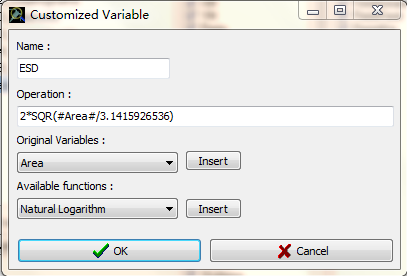
\includegraphics[width=0.7\textwidth]{CustomizedVariableWindow.png}
\caption{自定义变量窗口}
\label{fig: CustomizedVariableWindow}
\end{figure}

选中已存在的自定义变量,点击\textbf{Del}可以将其删除。

要新建一个自定义变量,点击\textbf{New},出现如图~\ref{fig: CustomizedVariableWindow}的变量自定义窗口。
\begin{enumerate}
\item 对新建的变量命名(命名必须与已有变量不同)
\item 在“Operation”下面一栏中输入计算公式
\item 按“OK”键
\end{enumerate}
{\color{blue}\textit{注:在编写公式时,一些基本的运算符(例如$+$, $-$, $\backslash$, $*$, $\^$)、括号、数字都是跟平常在键盘上敲的一样。要插入一个初始变量的话,可以在“Original Variables”下面一栏选中它,然后点击“Insert”。在公式中用到初始变量时,需要在这个初始变量前后加上“\#”号。在“Available functions”一栏中,可以选择一个函数进行插入。建议可以先看看已有的一些自定义变量是如何定义的,然后再编辑自己需要的公式。}}

4、Identification Groups(图~\ref{fig: EvaluationWindow}: {\color{red}\textbf{4}})

这里显示了在选取的学习文件中所定义的分类种类。默认的种类是不能被删除或编辑的,但是你可以通过将已有的类别合并来创建新的类别。

点击\textbf{New}可以创建新的类别,打开如图~\ref{fig: GroupsEditionWindow}所示的类别编辑窗口。

\begin{figure}[!ht]
\centering
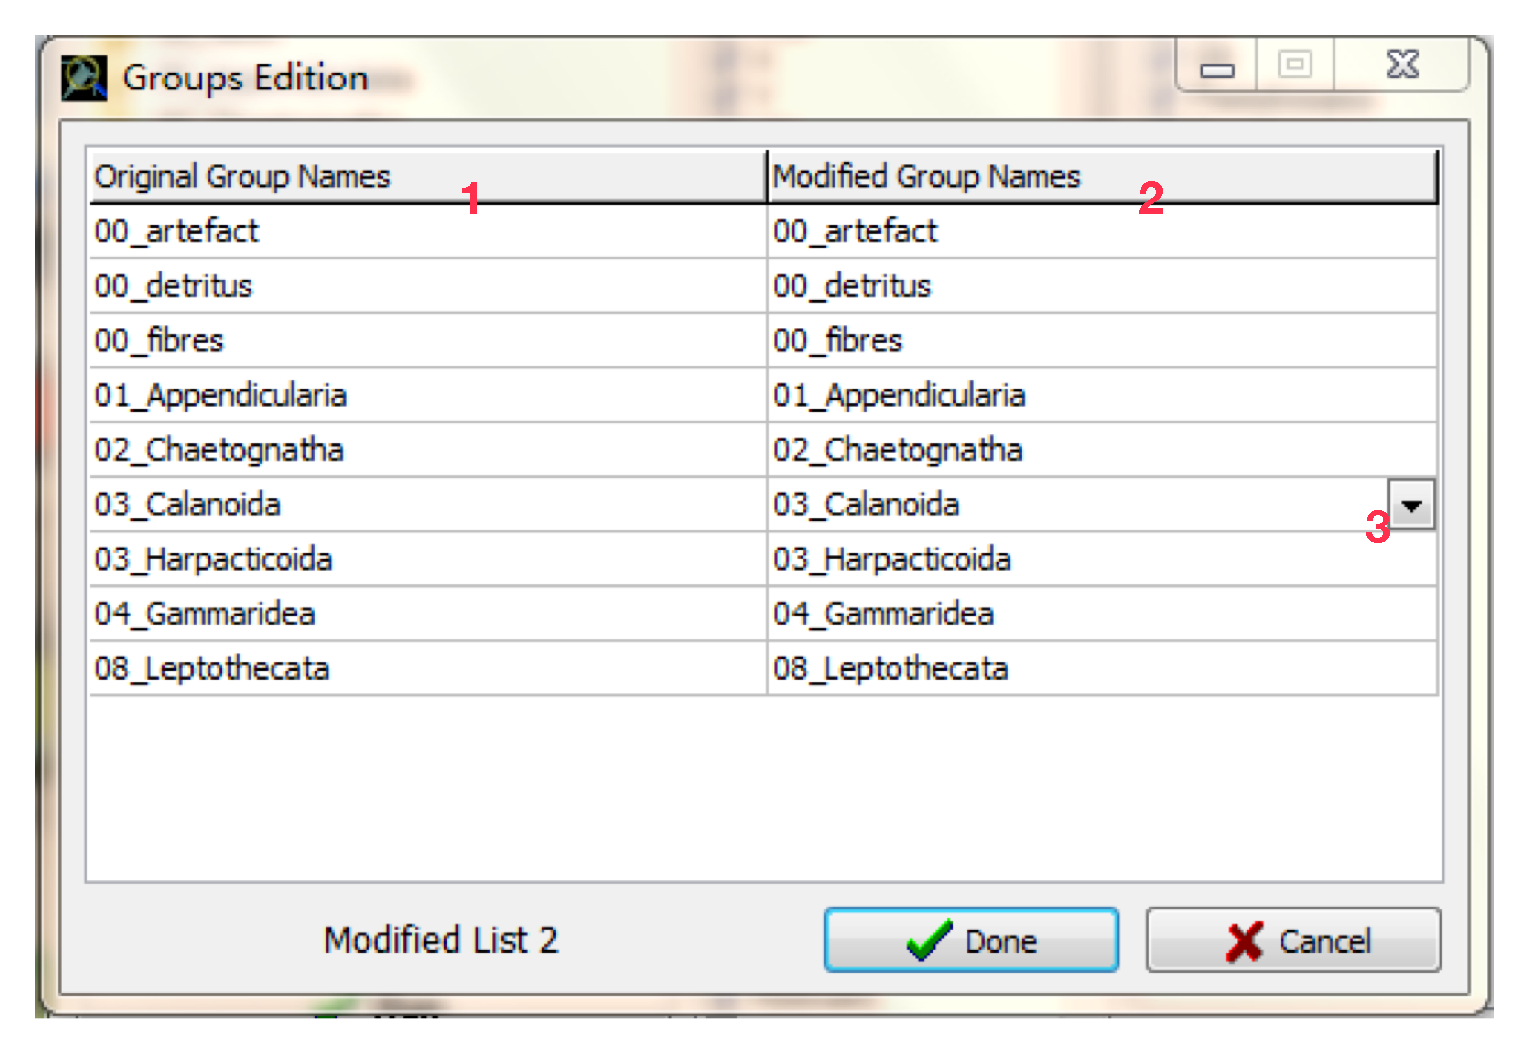
\includegraphics[width=0.7\textwidth]{GroupsEditionWindow.eps}
\caption{分类类别编辑窗口}
\label{fig: GroupsEditionWindow}
\end{figure}

修改初始类别名字(图~\ref{fig: GroupsEditionWindow}: {\color{red}\textbf{1}}):
\begin{enumerate}
\item 在“Modified Group Names”一栏下方选择一个需要修改的名字(图~\ref{fig: GroupsEditionWindow}: {\color{red}\textbf{2}})
\item 给这个类别重新编辑命名,或者点击如图(图~\ref{fig: GroupsEditionWindow}: {\color{red}\textbf{3}})所示按钮,在名字列表中选择一个
\item 完成对类别的重新命名后,点击\textbf{Done}
\end{enumerate}
{\color{blue}\textit{注:你可以创建很多的分类种类的列表,后续数据分析中用到的只会是当前这个列表(在Evaluation窗口点击\textbf{Run}时所看见的那个列表)。你可以用\textbf{Prev.}和\textbf{Next>}按钮来选择你想要的进行分析那个列表。在生成的结果文件中,初始名字会显示在“Ident1”这一列中,新的名字显示在“Ident2”这一列中。}}

5、选择一种方法(图~\ref{fig: EvaluationWindow}: {\color{red}\textbf{5}})

这里是要选择一种评价方法,用来检测用有监督学习方法和所选择的学习文件学习的模型的识别能力。PkID中一共提供了两种评价方法。

{\color{red}k-fold cross-validation method}:用重采样技术来评价学习算法在学习文件上的识别准确率。初始的训练数据集被随机分为$k$个相同大小的子集。每一次循环过程中,将$k-1$个子集放在一起形成训练集,并且构造出预测模型,剩下的那1个子集被当成测试集来评价模型预测能力。一共循环$k$次。这样下来,每个子集都会有1次机会作为测试集,$k-1$次机会作为训练集。将$k$次预测结果取平均,可以得到这个模型的最终预测能力。交叉验证过程会重复$n$次,$n$次交叉验证的平均错误率在一个混淆矩阵中被计算得到。

PkID一共实现了8种交叉验证方法,每一个都采用了不同的学习算法。

所有的交叉验证方法中所用的参数都是$k = 2, n = 5$。要想改变这两个值:

\begin{figure}[!ht]
\centering
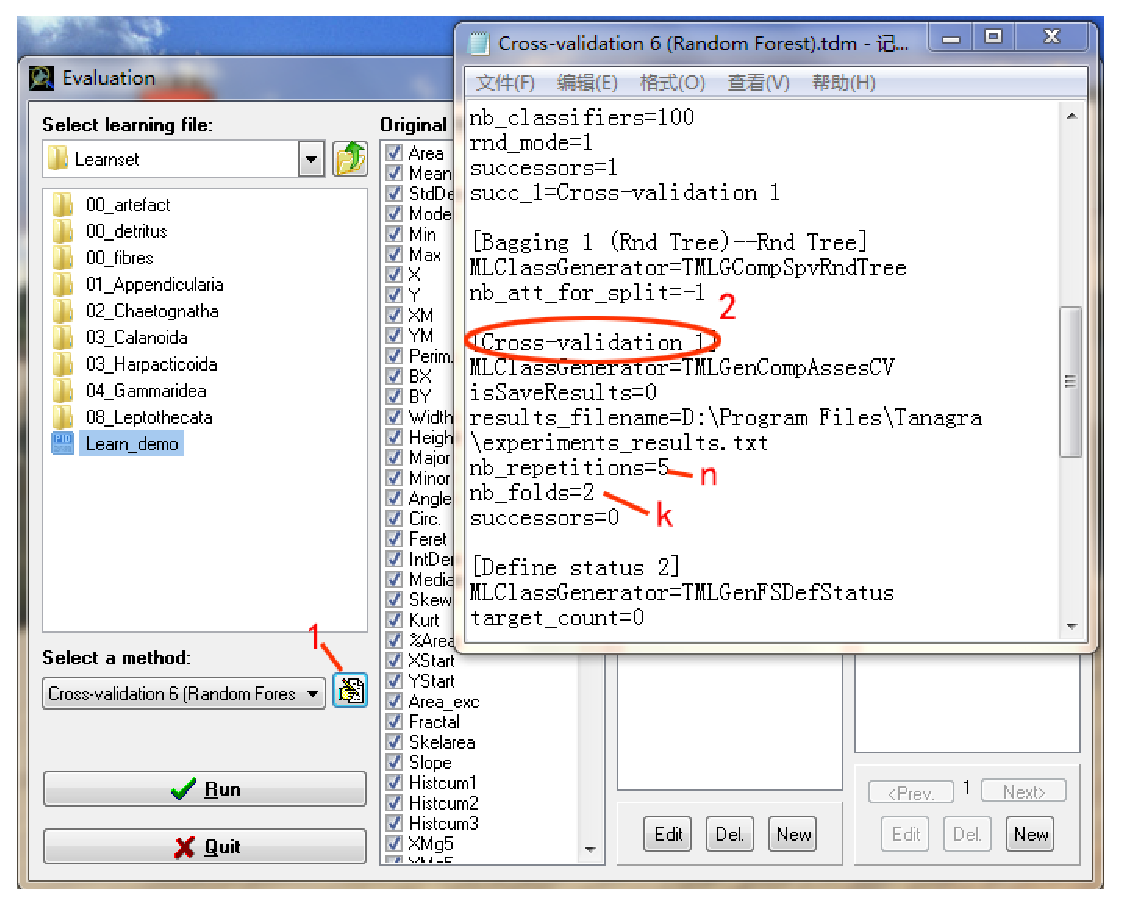
\includegraphics[width=0.7\textwidth]{ModificationofCrossValidationParameterisation.eps}
\caption{分类类别编辑窗口}
\label{fig: ModificationofCrossValidationParameterisation}
\end{figure}

\begin{enumerate}
\item 点击编辑按钮(图~\ref{fig: ModificationofCrossValidationParameterisation}: {\color{red}\textbf{1}}),打开相应的tdm文件
\item 在交叉验证部分修改$k$和$n$值图~\ref{fig: ModificationofCrossValidationParameterisation}: {\color{red}\textbf{2}}
\item 在关闭tdm文件前保存修改
\end{enumerate}

{\color{red}Test method}:在一个预先定义好的、独立的测试文件上对模型的准确率进行评价。在使用这个测试方法之前,需要创建一个特殊的文件,可以通过主窗口菜单中的\textbf{Concatenate Learning Files}来创建。相比于用两个不同的文件来作为训练集和测试集,我们更倾向于用一个文件来把它们联系起来,并且通过状态来表示所要扮演的角色,状态有“学习”和“测试”两种。

PkID提供了两种测试方法。Test 1可以通过在预先定义的测试文件上比较8个算法的准确率来选择最好的学习方法。Test 2只用到随机森林算法。

{\color{blue}\textit{注:通常来讲,训练集越大,所构造的分类模型越好,测试集越大,预测准确率越高。}}

{\color{red}Export to text file (no analysis)}:生成一个文本文件,包含了所选的学习文件中所有初始变量和自定义变量,而不包含预测结果。这个文件还可以输入到任意的数据挖掘软件站进行分析。

6、开始分析

当所有文件、变量、类别都选择好之后,点击\textbf{Run}按钮,将会出现一个保存页面,选择要保存的文件夹、文件名,点击\textbf{Save}。

分析完成后(可能需要几分钟,这取决于样本大小和所选方法),结果和html报告被保存在了所选择的文件夹中,并且html报告会自动在网页中打开。这时会有一个会话框询问你是否要退出Evaluation窗口,如果你选择“Yes”,Evaluation窗口就会被关闭并返回主窗口。

与初始PID文件相比,评价文件包含了以下新的列:
\begin{enumerate}
\item 对应于自定义变量的列
\item 包含了学习文件中分类类别的一列(Ident)
\item 包含了修改后的类别名字的一列(Ident2)
\item 用来表示状态的一列(Learning或Test)
\end{enumerate}

\subsection{Prediction}

这一步是要根据选择的学习文件中的种类对样本进行自动识别。结束后也会生成一个包含了自动识别结果的文本文件和一个包含了数据分析信息html报告。点击主窗口中的\textbf{Prediction}按钮,会打开一个新的窗口(图~\ref{fig: PredictionWindow}):

\begin{figure}[!ht]
\centering
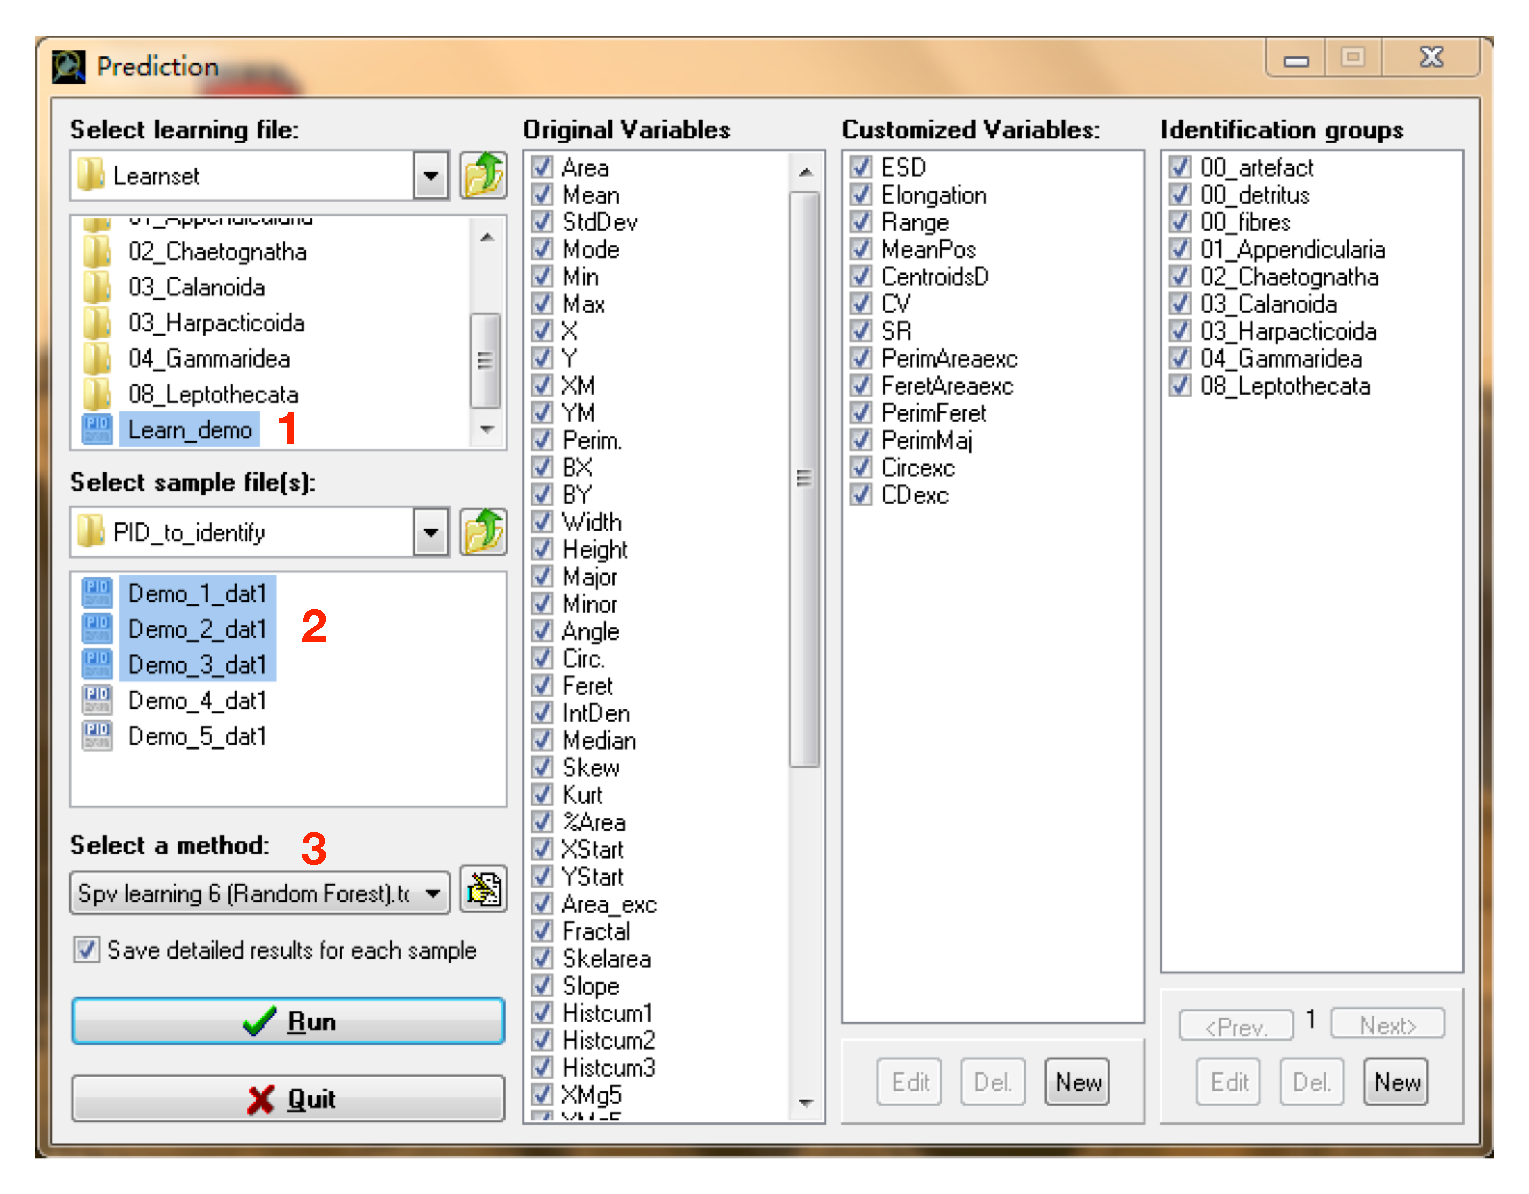
\includegraphics[width=0.7\textwidth]{PredictionWindow.eps}
\caption{Prediction窗口}
\label{fig: PredictionWindow}
\end{figure}

1、选择学习文件(图~\ref{fig: PredictionWindow}: {\color{red}\textbf{1}})

2、选择样本文件(图~\ref{fig: PredictionWindow}: {\color{red}\textbf{2}})

3、选择学习算法(图~\ref{fig: PredictionWindow}: {\color{red}\textbf{3}})

从PkID提供的8个学习算法中选择一个。
\begin{itemize}
\item Spv learning 1 (5-NN)
\item Spv learning 2 (C-SVC linear)
\item Spv learning 3 (C-SVC RBF)
\item Spv learning 4 (BVM)
\item Spv learning 5 (C4.5)
\item Spv learning 6 (Random Forest)
\item Spv learning 7 (PLS)
\item Spv learning 8 (Multilayer Perceptron)
\end{itemize}

4、开始分析

当所有文件、变量和分类类别都选好之后,点击\textbf{Run}按钮,会出现一个保存会话框。

\subsection{Validation}

这一步是将上一步生成的预测文件可视化,并且人为地对识别结果进行校正。这里可以有两个选择(图~\ref{fig: ValidationWindow}):1)用Prediction那一步生成的Pred\_.txt文件来将预测结果可视化,真正实现缩略图的自动分类,你还可以对自动识别的结果进行进一步检查和校正。2)打开一个已有的校正集来继续一个校正或进行二次校正。

\begin{figure}[!ht]
\centering
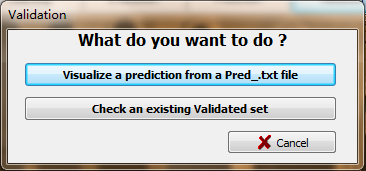
\includegraphics[width=0.7\textwidth]{ValidationWindow.png}
\caption{Validation窗口:What do you want to do?}
\label{fig: ValidationWindow}
\end{figure}

{\color{red}Visualize a prediction from a Pred\_.txt file}

\begin{figure}[!ht]
\centering
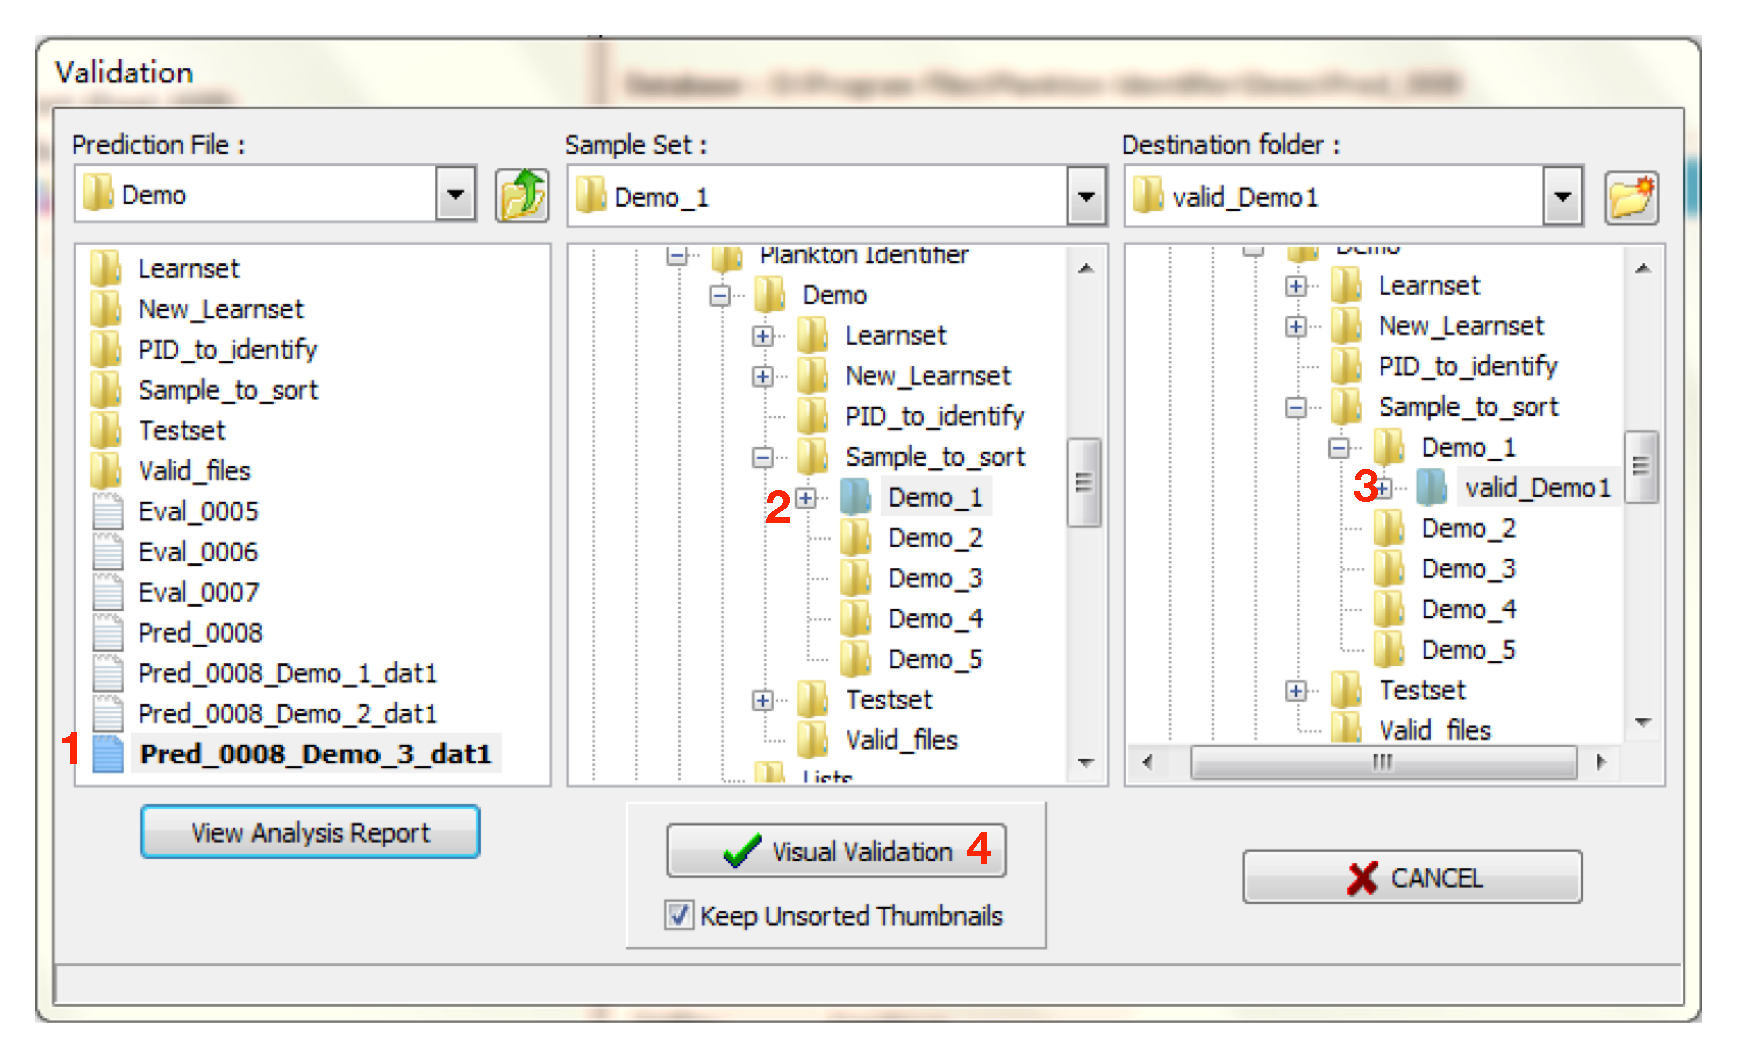
\includegraphics[width=0.7\textwidth]{SelectionWindowforValidation1.eps}
\caption{校正选择窗口1}
\label{fig: SelectionWindowforValidation1}
\end{figure}

\begin{enumerate}
\item 选择一个要用来校正的Pred\_.txt文件(图~\ref{fig: SelectionWindowforValidation1}: {\color{red}\textbf{1}})
\item 选择一个包含未分类缩略图的文件夹作为“Sample Set”(图~\ref{fig: SelectionWindowforValidation1}: {\color{red}\textbf{2}})
\item 选择用来存放分类好了的缩略图的目标文件夹(图~\ref{fig: SelectionWindowforValidation1}: {\color{red}\textbf{3}})
\item 点击“Visual Validation”(图~\ref{fig: SelectionWindowforValidation1}: {\color{red}\textbf{4}})
\end{enumerate}

{\color{blue}\textit{注:在分类过程中,缩略图是被复制而不是剪切到了目标文件夹中。如果你不想保留未分类的缩略图,可以在图~\ref{}处取消勾选\textbf{Keep Unsorted Thumbnails}。}}

{\color{red}Check an existing Validated set}

\begin{figure}[!ht]
\centering
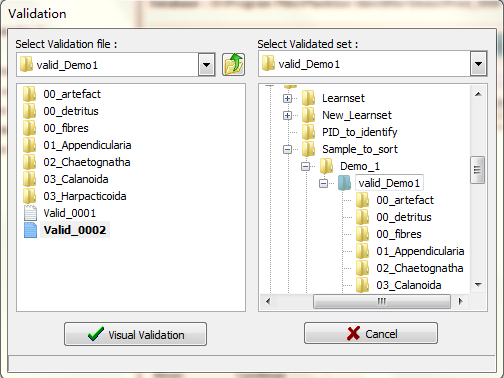
\includegraphics[width=0.7\textwidth]{SelectionWindowforValidation2.eps}
\caption{校正选择窗口2}
\label{fig: SelectionWindowforValidation2}
\end{figure}

\begin{enumerate}
\item 选择你想要检查的Valid\_.txt文件(图~\ref{fig: SelectionWindowforValidation2}: {\color{red}\textbf{1}})
\item 选择一个包含已分类好的校正后的缩略图的文件夹(图~\ref{fig: SelectionWindowforValidation2}: {\color{red}\textbf{2}})
\item 点击“Visual Validation”按钮(图~\ref{fig: SelectionWindowforValidation2}: {\color{red}\textbf{3}})
\end{enumerate}

{\color{red}Visual Validation}

前面的两个选择最终都会打开如图~\ref{fig: ValidationWindow2}所示的校正窗口:

\begin{figure}[!ht]
\centering
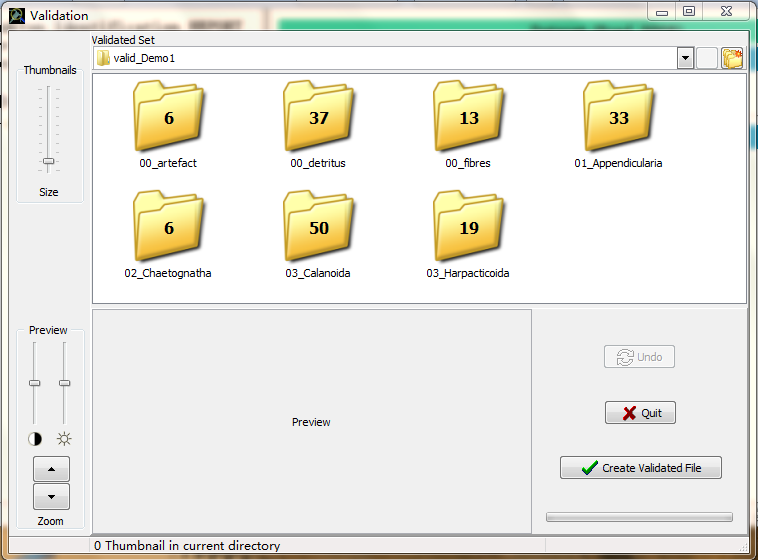
\includegraphics[width=0.7\textwidth]{ValidationWindow2.png}
\caption{校正窗口}
\label{fig: ValidationWindow2}
\end{figure}

利用预测模型已经将每幅缩略图放到了其对应的类别文件夹中,你可以打开每个文件夹查看是否被正确分类了。

{\color{red}Thumbnails moving}

\subsection{Compilation}

这一步是用来将上一步的生成的多个校正文件连起来,并且计算每个类别中的物体数目。在主窗口中点击\textbf{Compilation},会出现如下窗口(图~\ref{fig: CompilationWindow1}):

\begin{figure}[!ht]
\centering
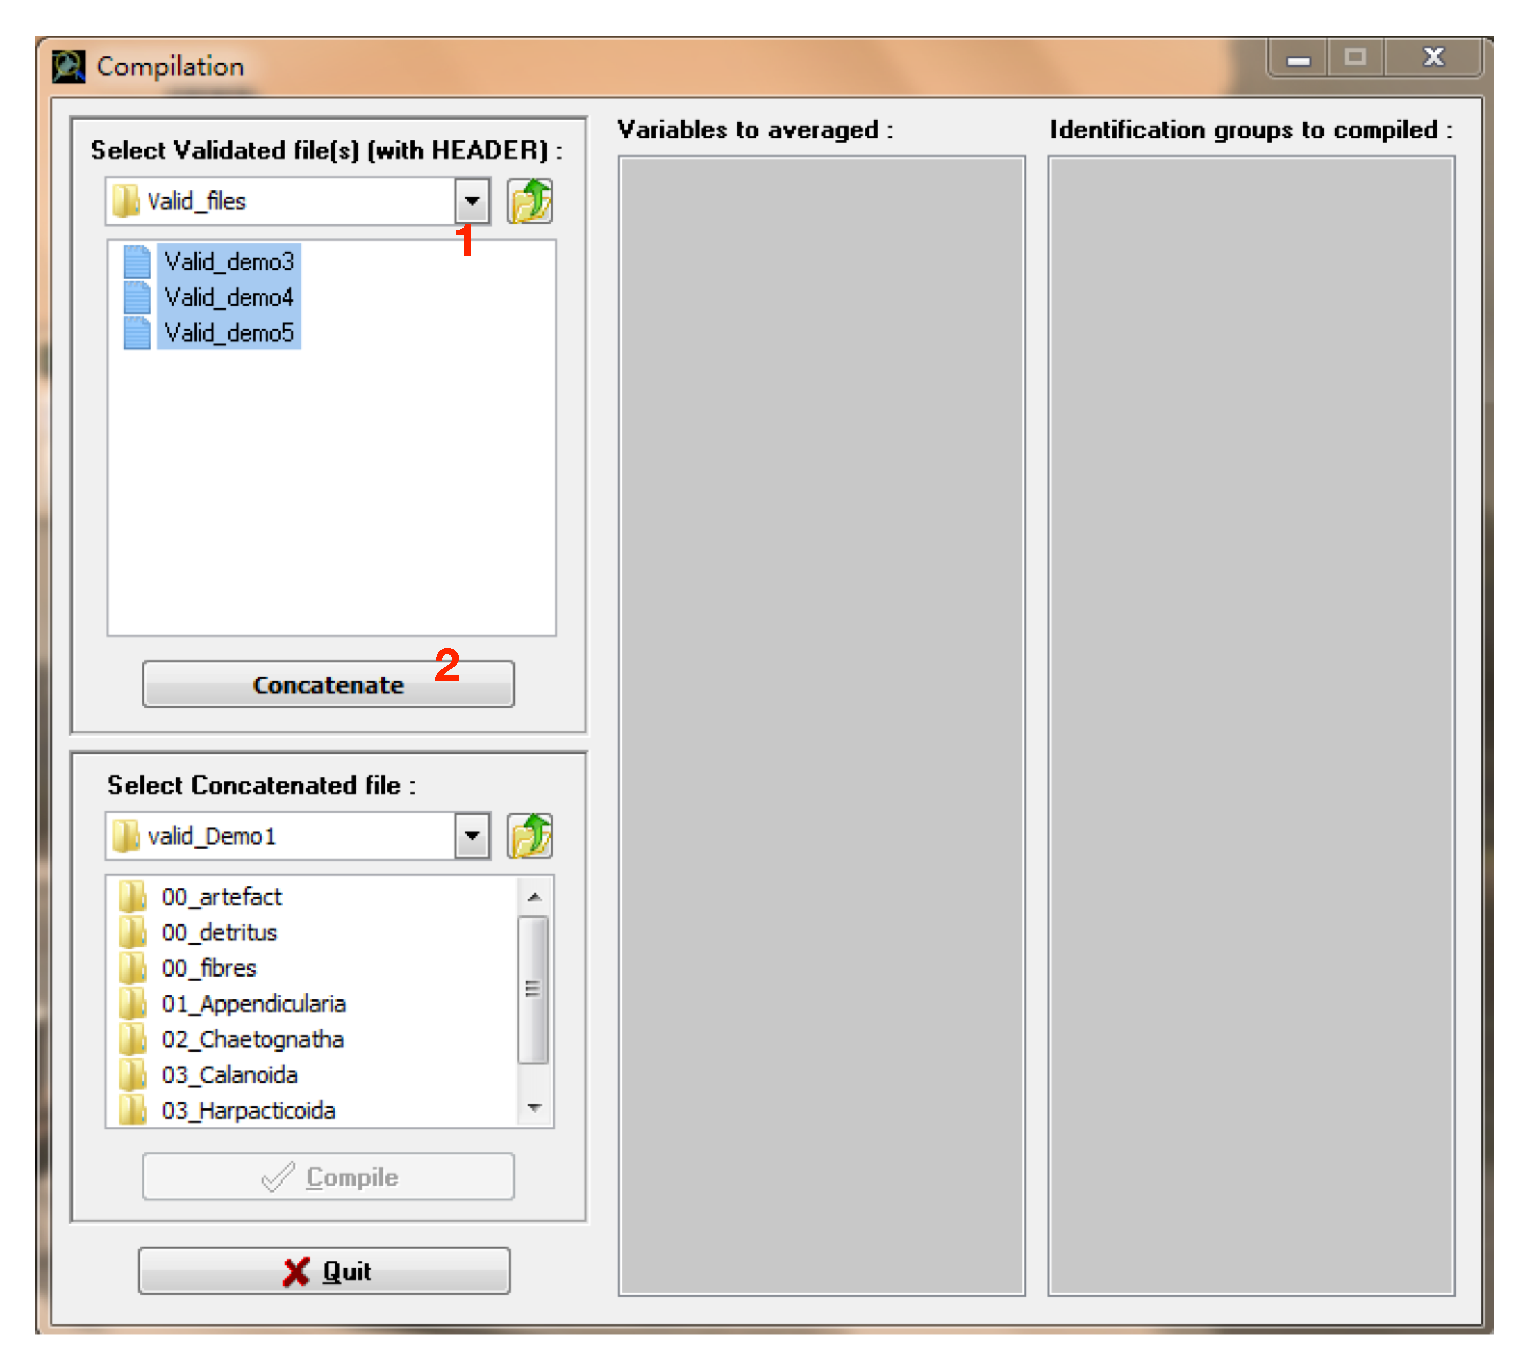
\includegraphics[width=0.7\textwidth]{CompilationWindow1.eps}
\caption{Compilation窗口:连接}
\label{fig: CompilationWindow1}
\end{figure}

1、Create a concatenation file

\begin{enumerate}
\item 浏览硬盘文件夹,找到包含你所要连接的Valid\_.txt文件的文件夹(图~\ref{fig: CompilationWindow1}: {\color{red}\textbf{1}})
\item 点击\textbf{Concatenate}(图~\ref{fig: CompilationWindow1}: {\color{red}\textbf{2}}),会出现一个保存会话框
\item 给连接后的文件进行命名,选择将其保存的文件夹路径
\item 点击\textbf{Save}按钮,连接就开始了(这可能需要几分钟,取决于你想要连接的文件数目)
\end{enumerate}

{\color{blue}\textit{注:要一次连接很多Valid\_.txt文件,需要把它们放在同一个文件夹中,然后按“Ctrl”键同时选中它们。}}

{\color{red}Create a compilation file}

\begin{figure}[!ht]
\centering
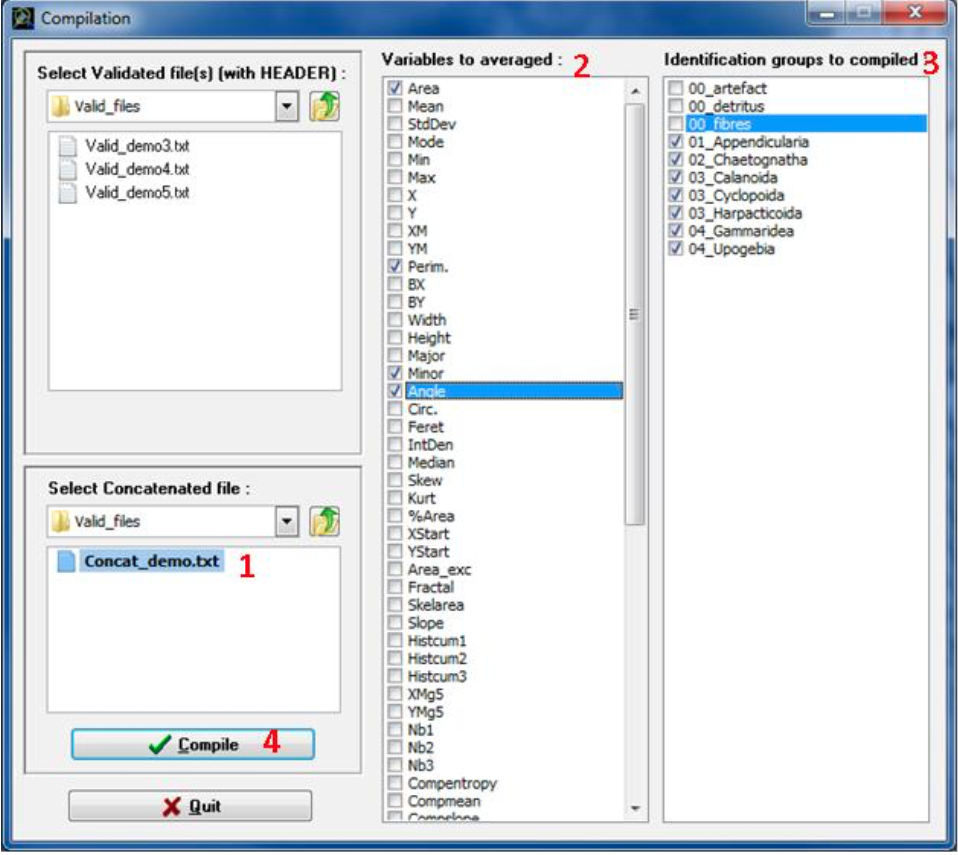
\includegraphics[width=0.7\textwidth]{CompilationWindow2}
\caption{Compilation窗口:编译}
\label{fig: CompilationWindow2}
\end{figure}

\begin{enumerate}
\item 选择一个已经连接好的Concat\_.txt文件。最终的连接文件会以粗体显示(图~\ref{fig: CompilationWindow2}: {\color{red}\textbf{1}})。
\item “Variables to averaged”一栏中可以勾选也可以不勾选相应的变量(图~\ref{fig: CompilationWindow2}: {\color{red}\textbf{2}}),被打上勾的变量在编译文件中会被平均,没有打勾的会被去除。
\item “Identification groups to compiled”一栏也可以挑选相应的类别打上勾(图~\ref{fig: CompilationWindow2}: {\color{red}\textbf{3}}),只有打上勾的类别才会计算出它所包含的物体数目。
\item 点击\textbf{Compile}按钮(图~\ref{fig: CompilationWindow2}: {\color{red}\textbf{4}}),出现一个保存会话框
\item 给编译后的文件进行命名,选择将其保存的文件夹路径
\item 点击\textbf{Save},编译就开始了
\end{enumerate}

编译后生成的文件如图~\ref{fig: CompilationFile}。

\begin{figure}[!ht]
\centering
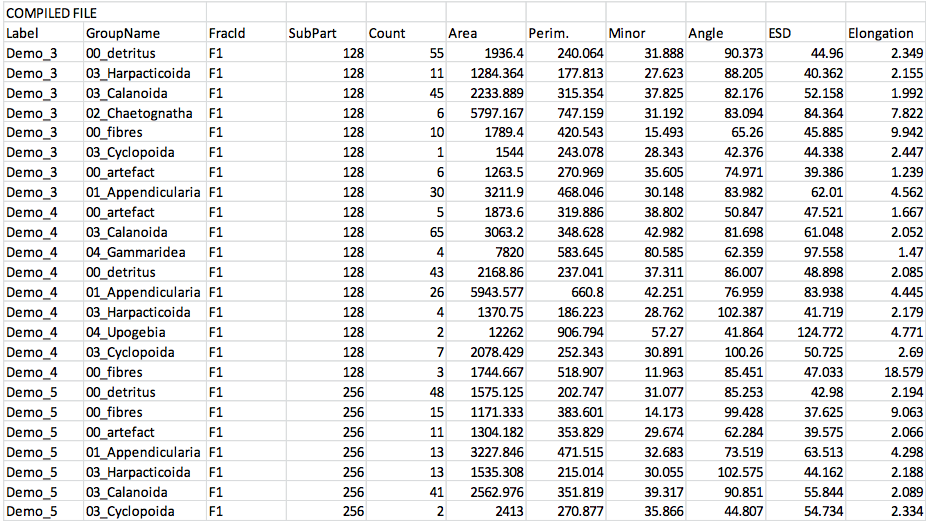
\includegraphics[width=0.7\textwidth]{CompilationFile}
\caption{编译文件}
\label{fig: CompilationFile}
\end{figure}
